\documentclass[12pt,letterpaper]{article}

% El archivo configuracion.tex tiene todos los paquetes a usar y los nuevos comandos que requiera


% Para escribir tildes y eñes
\usepackage[utf8]{inputenc}   %si compilo con lulatex no requiero este paquete


 % Activate to begin paragraphs with an empty line rather than an indent
 \usepackage[parfill]{parskip}


%borra los espacios verticales por defecto que usa LaTex
\raggedbottom


% Para usar el ambiente enumerate
\usepackage{enumerate}


% Para que los títulos de figuras, tablas y otros estén en español
\usepackage[spanish,es-noquoting]{babel} 
	% Cambiar nombre a tablas
	\addto\captionsspanish{\renewcommand{\tablename}{Tabla}}	
    % Cambiar nombre a lista de tablas		
	\addto\captionsspanish{\renewcommand{\listtablename}{Índice de tablas}}	
    % Cambiar nombre a capítulos
	\addto\captionsspanish{\renewcommand{\chaptername}{Sección}}

% Para que la bibligrafía esté en español
\usepackage{babelbib}

% Tamaño del área de escritura de la página	
\usepackage{geometry}                         
	%\geometry{left=18mm,right=18mm,top=23mm,bottom=23mm,headheight=15pt} 	

% Paquetes para matemática
%%%%%%%%%%%%%%%%%%%%%%%%%%%%%%%

% Los paquetes ams son desarrollados por la American Mathematical Society y mejoran la escritura de fórmulas y símbolos matemáticos.
\usepackage{amsmath} %Permite hacer presentación de ecuaciones      
\usepackage{amsfonts}     	
\usepackage{amssymb}
\usepackage{mathtools}


% Paquetes para manejo de gráficas y figuras
%%%%%%%%%%%%%%%%%%%%%%%%%%%%%%%

% Para insertar gráficas
\usepackage{graphicx}     	

% Para colocar varias subfiguras
\usepackage[lofdepth,lotdepth]{subfig}

% Para crear gráficos vectoriales con un lenguaje descriptivo/geométrico
\usepackage{tikz}

% Para crear circuitos vectoriales basados en TikZ
\usepackage[american]{circuitikz}

% Para crear gráficas en tikz
\usepackage{pgfplots}
\pgfplotsset{compat=1.15}

% Paquetes relacionados con el estilo 
%%%%%%%%%%%%%%%%%%%%%%%%%%%%%%%

% Para la presentación correcta de magnitudes y unidades
\usepackage{siunitx}	

% Para hipervínculos y marcadores
\usepackage[colorlinks=true,urlcolor=blue,linkcolor=black,citecolor=blue]{hyperref}
	\urlstyle{same}
\usepackage{cite}



% Para ubicar las tablas y figuras justo después del texto
\usepackage{float}	

% Para hacer tablas más estilizadas
\usepackage{booktabs}		

% Para hacer secciones con múltiples columnas
\usepackage{multicol} %me permite crear columnas entre las paginas sin generar espacios en blanco, pero no permite objetos flotantes

%*************CONSTRUCCION DE NUEVOS COMANDOS*************%
%\renewcommand{\columnseprule}{0.5pt} %genera una linea entre las columnas que creo en el documento


%*************CONFIGURACION DE COMANDOS*************%
%\setlength\columnsep{20mm} %Separación entre columnas


% Para utilizar el número de páginas
\usepackage{lastpage}

% Para manejar los encabezados y pies de página
%\usepackage{fancyhdr}
	% Contenido de los encabezados y pies de pagina
%	\pagestyle{fancy}
  % Los encabezados los configuro en el main.tex

% Misceláneos
%%%%%%%%%%%%%%%%%%%%%%%%%%%%%%%

% Para insertar símbolos extraños
\usepackage{marvosym}
\usepackage{lscape}
\usepackage{upgreek}%Para usar tao


% Para generar texto aleatorio
\usepackage{lipsum}


\usepackage{verbatim} % Sirve para usar el ambiente de comentarios \begin{comment} o \verb+ <xxxx> +


% Para agregar los colores al documento
\usepackage{xcolor}
\usepackage{color}


% Para agregar código con formato de Matlab
%\usepackage[numbered,autolinebreaks]{mcode} %requiere tener el archivo mcode.sty

% Para insertar código fuente estilizado
\usepackage{listings}

\definecolor{miverde}{rgb}{0,0.6,0}
\definecolor{migris}{rgb}{0.5,0.5,0.5}
\definecolor{mimalva}{rgb}{0.58,0,0.82}

\lstset{ %
  backgroundcolor=\color{white},   % Indica el color de fondo; necesita que se añada \usepackage{color} o \usepackage{xcolor}
  basicstyle=\ttfamily,        % Fija el tamaño del tipo de letra utilizado para el código, otro puede ser \ttfamily, \footnotesize
  breakatwhitespace=false,         % Activarlo para que los saltos automáticos solo se apliquen en los espacios en blanco
  breaklines=true,                 % Activa el salto de línea automático
  captionpos=b,                    % Establece la posición de la leyenda del cuadro de código
  commentstyle=\color{miverde},    % Estilo de los comentarios
  deletekeywords={...},            % Si se quiere eliminar palabras clave del lenguaje
  escapeinside={\%*}{*)},          % Si quieres incorporar LaTeX dentro del propio código
  extendedchars=true,              % Permite utilizar caracteres extendidos no-ASCII; solo funciona para codificaciones de 8-bits; para UTF-8 no funciona. En xelatex necesita estar a true para que funcione.
  frame=single,	                   % Añade un marco al código
  keepspaces=true,                 % Mantiene los espacios en el texto. Es útil para mantener la indentación del código(puede necesitar columns=flexible).
  keywordstyle=\color{blue},       % estilo de las palabras clave
  language=c,                 	   % El lenguaje del código
  otherkeywords={*,...},           % Si se quieren añadir otras palabras clave al lenguaje
  numbers=none,                    % Posición de los números de línea (none, left, right).
  numbersep=5pt,                   % Distancia de los números de línea al código
  numberstyle=\small\color{migris}, % Estilo para los números de línea, otro puede ser \tiny,
  rulecolor=\color{black},         % Si no se activa, el color del marco puede cambiar en los saltos de línea entre textos que sea de otro color, por ejemplo, los comentarios, que están en verde en este ejemplo
  showspaces=false,                % Si se activa, muestra los espacios con guiones bajos; sustituye a 'showstringspaces'
  showstringspaces=false,          % subraya solamente los espacios que estén en una cadena de esto
  showtabs=false,                  % muestra las tabulaciones que existan en cadenas de texto con guión bajo
  stepnumber=2,                    % Muestra solamente los números de línea que corresponden a cada salto. En este caso: 1,3,5,...
  stringstyle=\color{mimalva},     % Estilo de las cadenas de texto
  tabsize=2,	                   % Establece el salto de las tabulaciones a 2 espacios
  title=\lstname                   % muestra el nombre de los ficheros incluidos al utilizar \lstinputlisting; también se puede utilizar en el parámetro caption
}

 



\begin{document}

%***************************PORTADA***********************************

\begin{titlepage}
    \begin{center}
        \vspace*{1cm}
            
        \Huge
        \textbf{Nociones de la memoria del computador \textcolor{red}{\Biohazard}}
            
        \vspace{0.5cm}
        \LARGE
        %Subtítulo
            
        \vspace{1.5cm}
            
        \textbf{Diego Alejandro Londoño Jiménez\\ \emph{diegoa.londono@udea.edu.co} }
            
        \vfill
            
        \vspace{0.8cm}
            
        \Large
        Despartamento de Ingeniería Electrónica y Telecomunicaciones\\
        Universidad de Antioquia\\
        Medellín\\
        Septiembre de 2020\\
        
            
    \end{center}
\end{titlepage}


%***************************FIN PORTADA***********************************

\tableofcontents


\newpage

\section{Introducción}

En la solución del taller se describirá los tipos de memoria que usa un computador para su funcionamiento, esta descripción se dará en las respuestas que ha planteado el profesor para la realización del taller.

En el desarrollo del taller se encontraran preguntas del tipo: Defina, mencione, describa, esto con el fin de simplificar el artículo propuesto por el profesor.

Al final cuando el usuario termine de leer las respuestas del taller, se espera que pueda entender de manera muy básica que es el funcionamiento de la memoria en el computador.


\newpage


\section{Preguntas del taller.}\label{preguntas}
    \subsection{Defina que es la memoria del computador.}

La memoria es uno de los componentes que hace parte del computador, en dicho componente se almacena la información a procesar. La información que este componente procesará puede ser fija o volátil, fija es aquella que al momento de apagar el computador ella no desaparece y volátil cumple lo contrario a lo explicado anteriormente.

Si el usuario desea que su información no se pierda al momento de apagar su computadora, esta se debe de almacenar en la memoria \textbf{\emph{rom}}, mientras que la memoria \textbf{\textit{RAM}} se encarga de almacenar información volátil.

\begin{quote}
    ``La memoria cumple un papel muy importante en el computador y su funcionamiento, ya que se
    trata del dispositivo donde se almacena temporalmente toda la información con la que trabajan
    los microprocesadores para procesarla y devolver los resultados que los usuarios requieren.''\cite{GuiaProfesor}
\end{quote}

\subsection{Mencione los tipos de memoria que conoce y haga una pequeña descripción de cada tipo.}

Entre los varios tipos de memoria que se manejan para los sistemas embebidos\footnote{\url{https://n9.cl/y6ac}} o para los computadoras, en este taller sólo se explicaran las mencionadas en el artículo suministrado por el profesor.\footnote{\tiny{\url{http://www.youbioit.com/es/article/shared-information/8714/como
-funciona-la-memoria-de-una-computadora}}}

\begin{itemize}
    \item Memoria Cache L1,L2,L3
    \item Memoria RAM
    \item Memoria Swap
    \item Memoria ROM
\end{itemize}

Se empezará a describir la memoria de mayor rapidez a su acceso pero siendo inversamente proporcional a su tamaño de almacenamiento.


La memoria \textbf{\textit{cache}}, esta es la de menor tamaño comparada con el resto de memorias que maneja el computador, pero es la más rápida de todas, dado que su ubicación se encuentra dentro del microprocesador, observar la figura \ref{F:versus}

\begin{figure}[H]
    \centering
    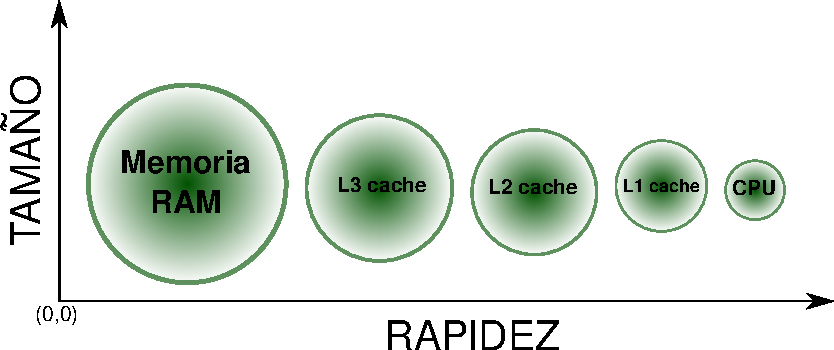
\includegraphics[angle=0]{image/MemoriaCache.pdf}
    \caption{Tamaño vs Rapidez}
    \label{F:versus}
\end{figure}


\textbf{Memoria Cache L1,L2,L3}: La memoria \textbf{\textit{cache}} maneja tres niveles L1,L2,L3, de estos niveles se puede decir que entre más alto el coeficiente numérico es menor su tamaño de almacenamiento y entre más pequeño el coeficiente numérico, mas rápida es la memoria. Lo anterior se puede ver graficamente en la figura \ref{F:versus}.

\begin{quote}
     ``La memoria Cache se utiliza para trabajar con los datos e instrucciones que el microprocesador ve que se utilizan más seguido, entonces para no tener que ir a buscarlos una y otra vez de la memoria RAM que es más lenta, coloca una copia de esos datos en la memoria Cache para tenerlos a mano.''\cite{GuiaProfesor} 
\end{quote}

\textbf{Memoria RAM (Random Access Memory):} Esta memoria se encuentra ubicada fuera del microprocesador, por lo tanto hace que su acceso a ella sea mas lenta comparada con la memoria \textbf{\textit{cache}}, su tamaño de almace es mucho mas grande que la memoria \textbf{\textit{cache}}. Se debe tener presente que al momento de formatear un computador, el sistema operativo no se reinstala él mismo, por lo tanto este procedimiento se hace cargando todo el sistema operativo en la memoria \textbf{\textit{RAM}} y desde allí se ejecuta la nueva instalación deseada.

Lo mencionado anteriormente es considerado como una de las varias funciones de la memoria \textbf{\textit{RAM}}, dado que ella tiene más funciones durante el encendido del computador.

\begin{quote}
    ``La memoria RAM es el tipo de memoria más importante del computador, su nombre representa las siglas de Random Access Memory (Memoria de Acceso Aleatorio); la razón de dicho nombre es porque la misma está dividida en celdas de memoria donde se almacenan cada uno de los bits o pulsos eléctricos (que representan los 1 y 0) y a las cuales se puede acceder directamente indistintamente de su posición o dirección.''\cite{GuiaProfesor}
\end{quote}

\textbf{Memoria Swap}: Conocida como la unidad de intercambio\footnote{\url{https://wiki.archlinux.org/index.php/Swap_(Espa\%C3\%B1ol)}}, esta memoria se encuentra en un espacio de asignado del disco duro en el momento de la instalación del sistema operativo o en un momento posterior. Una de sus funciones es dar apoyo a la memoria \textbf{\textit{RAM}} en el momento que se está se está quedando sin espacio de memoria

\begin{quote}
    ``Simplemente sirve para ``sostener'' porciones de un progRAMa que no se está utilizando ``todavía'' pero que en cualquier momento sí se utilizará; y que dado que el disco duro es mucho más lento que la memoria \textbf{\textit{RAM}} no es bueno depender mucho de ella.''\cite{GuiaProfesor}
\end{quote}


\textbf{Memoria ROM} (Read Only Memory)Sirve para almacenar los progRAMas instalados y SO, entre otras funciones. En el momento que esta se apaga, no es pierde la información guardada en ella

        
\subsection{Describa la manera como se gestiona la memoria en un computador}
    La memoria RAM almacena información o instrucciones para ser usada por el microprocesador, en el momento que esta información no se requiere dicha información es borrada del espacio de memoria, lo mismo sucede en el momento que la instruccion es usada por el microprocesador, esta es borrada para liberar espacio en dicha memoria. El encargado de realizar dicha función es el controlador de memoria.       


\subsection{¿Qué hace que una memoria sea más rápida que otra? ¿Por qué esto es importante?}
    La rapidez de la memoria depende de la cercania fisica a la CPU, dependiendo de la rapidez, se elegirá en que memoria almacenar la información requerida 
        
\newpage

\section{Conclusiones}
    \begin{itemize}
        \item A medida que la memoria esté mas cerca de la CPU su velocidad aumenta.
        \item La velocidad es inversamente proporcial al tamaño en byte.
        \item Entre más grande el tamaño de la memoria comparada con la memoria que está mas cerca a la CPU, su valor económico es más favorable.
        \item Entre más memoria RAM, mayor consumo energetico, esto ultimo por la forma de cómo cargada de información o instrucciones la memoria RAM
    \end{itemize}

\newpage

\bibliographystyle{IEEEtran}
\bibliography{references}

\end{document}
